\documentclass[../thesis.tex]{subfiles}
% Separate preamble for this subfile. This preamble is loaded last, so it may be used to override various functions.

% Better comment extension for Vscode colors these comments differently
% Normal comment color
% * Important information is highlighted
% ! ALERT
% ? Question
% TODO stuff to do
% // this is strikethrough


\begin{document}
In \cite{jorgensenSpectralPairsCartesian2001}, Pedersen and Jorgensen present a way of constructing spectral pairs in higher dimensions from spectral pairs in lower dimensions. 
\SigridComment{Innføre en mer distinkt notasjon på $\Lambda(\lambda_1)$, for å skille den fra et settet lambda, det har i hvertfall vært en smule forvirrende for min del. Ekempelvis, $\Lambda'(\lambda_1)$, men aller helst Lambda i en annen font: $\mathbf{\Lambda}(\lambda_1)$ eller $\mathsf{\Lambda}(\lambda_1)$ (ser den ikke printet noe her men det kan jeg se på)} 

\begin{equation*}
    \mathbf{\Lambda}(\lambda_1), \mathbf{\Lambda}(\lambda_1)
    \mathbf{L}(\lambda_1), \mathsf{L}(\lambda_1)
\end{equation*}

\begin{theorem}[Construction of spectra]\label{thrm:construction_spectra}
    Let $\brac{\Omega_1,\Lambda_1}$ be a spectral pair in dimension $d_1$, and let $\Omega_2$ be a set of positive finite measure in dimension $d_2$. Suppose for each $\lambda_1 \in \Lambda_1$ that $\Lambda(\lambda_1)$ is a discrete subset of $\R^{d_2}$ such that $\brac{\Omega_2,\Lambda(\lambda_1)}$ is a spectral pair. If 
    \begin{equation*}
        %\Lambda = \braq{\lambda: \lambda \in  \Lambda_1 \times \Lambda_2} = \braq{\brac{\lambda_1, \lambda_2}: \lambda_1\in \Lambda_1, \lambda_2 \in \Lambda_2} 
        \Lambda = \braq{\brac{\lambda_1, \lambda_2}: \lambda_1\in \Lambda_1, \lambda_2 \in \Lambda(\lambda_1)} 
    \end{equation*}
    then $\brac{\Omega_1\times\Omega_2, \Lambda}$ is a spectral pair in $d_1+d_2$ dimensions. 
\end{theorem}
% * In \cite{jorgensenSpectralPairsCartesian2001} Steen P. and Palle E. presented a method on the construction of spectral pairs in higher dimensions. It is a recursive technique in what they dub "a cross-product construction" using "factors" in lower dimensions, and applies for any two spectral pairs $\brac{\Omega_i,\Lambda_i}$ where $i=1,2$ and in arbitrary dimensions $d_1$ and $d_2$. The technique is presented in the following theorem
%[p.~3]
\SigridComment{Ja, Nei, ikke noe poeng å utbrodere?}
\begin{remark}
    It can be helpful to think of $\Lambda(\lambda_1)$ as a function that assigns a discrete subset to each $\lambda_1$-value such that $\brac{\Omega_2,\Lambda(\lambda_1)}$ is itself a spectral set at $\lambda_1$. That naturally also means the discrete set $\Lambda(\lambda_1)$ at $\lambda_1$ must be orthogonal to the original spectral set $\Lambda_1$. When representing this in a figure, one should note the similarity to a cross product of spaces such as $\Z \times \Z$ or $\R \times \R$. Most important in the construction of spectra presented \cref{thrm:construction_spectra} is that it opens up the possibility of having a different discrete set at each $\lambda_1$-value. This newfound flexibility will be discussed after the proof of the \namecref{thrm:construction_spectra}.
\end{remark} % Før "When representing" ha: Note that we would still have that the zero-element is the only element that is orthogonal to both sets.

\begin{proof}
    Given $\Lambda$ as constructed in \cref{thrm:construction_spectra}, we start by showing that the set of exponentials $E(\Lambda)$
    %\begin{equation}
    %    E(\Lambda) = \braq{e^{2\pi i \braa{\lambda, t} } : \lambda \in \Lambda_1\times\Lambda_2}
    %\end{equation}
    % given in \cref{eq:exp_set_all_d}
    is pairwise orthogonal in $L^2\brac{\Omega_1 \times \Omega_2}$. Using two elements $e_\lambda,e_{\lambda'} \in E(\Lambda)$ we have %the following inner product %Note that $t$ denotes the vector $(t_1,t_2)$ where $t_1 in \Omega_1$ and $t_2 \in \Omega_2$
    \begin{align*}
        \braa{e_\lambda,e_{\lambda'}}_{L^2\brac{\Omega_1 \times \Omega_2}} 
        &= \int_{\Omega_1} \int_{\Omega_2} e_{\lambda}(t) \overline{e_{\lambda'}(t)} dt_2 dt_1\\ 
        &= \int_{\Omega_1} \int_{\Omega_2} e^{2\pi i \braa{\lambda, t} } e^{-2\pi i  \braa{\lambda', t}} dt_2 dt_1\\ 
        &= \int_{\Omega_1} \int_{\Omega_2} e^{2\pi i \brac{\lambda_1 t_1+\lambda_2 t_2}} e^{-2\pi i\brac{\lambda_1' t_1+\lambda_2' t_2}} dt_2 dt_1\\ 
        &= \int_{\Omega_1} \int_{\Omega_2} e^{2\pi i \brac{\lambda_1- \lambda_1'}t_1} e^{2\pi i \brac{\lambda_2 - \lambda_2'}t_2} dt_2 dt_1\\ 
        &= \underbrace{\int_{\Omega_1} e^{2\pi i  \brac{\lambda_1- \lambda_1'}t_1}}_{\text{Outter}} \underbrace{\bracMed{\int_{\Omega_2}  e^{2\pi i \brac{\lambda_2 - \lambda_2'}t_2} dt_2}}_{\text{Inner}} dt_1
    \end{align*}
    Note that the entire integral will vanish if either the inner or outer integral is zero. If $\lambda_2 \neq \lambda_2'$, then as both $\lambda_2, \lambda_2' \in \Lambda(\lambda_1)$ the inner integral will be zero from the fact that $\brac{\Omega_2, \Lambda(\lambda_1)}$ is a spectral pair. Conversely, if $\lambda_2 = \lambda_2'$ the resulting integral will factor as % THE inner integral will be equal to $\mes{\Omega_2}$, and the resulting integral will be
    \begin{align*}
        = \mes{\Omega_2} \int_{\Omega_1} e^{2\pi i  \brac{\lambda_1- \lambda_1'}t_1} dt_1
    \end{align*}
    Now, if one assume $\lambda_1 \neq \lambda_1'$, then as both $\lambda_1, \lambda_1' \in \Lambda_1$ the (outter) integral will be zero from the fact that $\brac{\Omega_1, \Lambda_1}$ is a spectral pair. However, if $\lambda_1 = \lambda_1'$, observe that we have the case where $\lambda = \lambda'$, and that
    \begin{align*}
        \braa{e_\lambda, e_\lambda}_{L^2\brac{\Omega_1 \times \Omega_2}}
        &= \int_{\Omega_1} \int_{\Omega_2} e_{\lambda}(t) \overline{e_{\lambda}(t)} dt_2 dt_1
        =\int_{\Omega_1} \int_{\Omega_2} |e^{2 \pi i \lambda t}|^2 dt_2 dt_1
        = \int_{\Omega_1} \int_{\Omega_2} |1|^2 dt_2 dt_1\\
        &= \mes{\Omega_1}\mes{\Omega_2} \neq 0
    \end{align*}
    %\begin{align*}
    %    \mes{\Omega_2} \int_{\Omega_1} e^{2\pi i  \brac{\lambda_1- \lambda_1'}t_1} dt_1 
    %    = \mes{\Omega_2} \mes{\Omega_1} 
    %    = \braa{e_\lambda, e_\lambda}_{L^2\brac{\Omega_1 \times \Omega_2}}
    %    \neq 0
    %\end{align*}
    To show that $E(\Lambda)$ is complete in $L^2(\Omega_1 \times \Omega_2)$, let $f\in L^2\brac{\Omega_1 \times \Omega_2}$ and assume it is orthogonal to $\spn{E(\Lambda)}$. For all $e_\lambda \in E(\Lambda)$ the inner product similarly factors as
    \begin{align*} % REMEMBER t is a vector, i.e t=(t_1,t_2)
        \braa{e_\lambda,f}_{L^2\brac{\Omega_1 \times \Omega_2}}
        &= \int_{\Omega_1} \int_{\Omega_2} e_\lambda(t) \overline{f(t)} dt_2dt_1 \\
        &= \int_{\Omega_1} \int_{\Omega_2} e^{2\pi i  (\lambda_1 t_1 + \lambda_2 t_2)} \overline{f(t_1,t_2)} dt_2 dt_1 \\
        &= \int_{\Omega_1} e^{2 \pi i \lambda_1 t_1} \int_{\Omega_2}e^{2 \pi i \lambda_2 t_2} \overline{f(t_1,t_2)} dt_2 dt_1
        %&= 0
    \end{align*}
    If we fix $\lambda_2$, we denote the inner integral by 
    \begin{equation}\label{eq:inner_eq}
        F(t_1) := \int_{\Omega_2} e^{2 \pi i \lambda_2 t_2} \overline{f(t_1,t_2)} dt_2,
    \end{equation}
    and make a note that $F\in L^2(\Omega_1)$. We thus have % This allows us to rewrite our initial inner product into
    \begin{equation}\label{eq:outter_eq}
        \braa{e_{\lambda}, f}_{L^2(\Omega_1\times \Omega_2)} = \int_{\Omega_1} e^{2 \pi i \lambda_1 t_1} F(t_1) dt_1 = \braa{e_{\lambda_1}, F}_{L^2(\Omega_1)} = 0, \quad \text{ for all } \lambda_1 \in \Lambda_1 .
    \end{equation}
    Using the fact that $E(\Lambda_1)$ is complete in $L^2(\Omega_1)$, we have from \cref{lem:ONB_alternative_def} that $F(t_1)=0$ for almost every $t_1 \in \Omega_1$. Now as we must have \labelcref{eq:inner_eq} equal to zero, observe that since $\lambda_2$ was arbitrarily, and we know that $E(\Lambda(\lambda_1))$ is complete in $L^2(\Omega_2)$, then the same \namecref{lem:ONB_alternative_def} implies that $f=0$. Thus, $E(\Lambda)$ is complete in $L^2\brac{\Omega_1 \times \Omega_2}$ which finalizes the proof.
    %Using the fact that $E(\Lambda_1)$ is complete in $L^2(\Omega_1)$, we have from \cref{lem:ONB_alternative_def} and almost all $t_1 \in \Omega_1$, that the only element in $L^2(\Omega_1)$ that results in $\braa{e_{\lambda_1}, F} = 0$ for all $e_{\lambda_1} \in E(\Lambda_1)$ is the zero-element $F=0$. Now as we must have \cref{eq:inner_eq} equal to zero, observe that as we fixed $\lambda_2$ arbitrarily, and we know that $E(\Lambda_2)$ is complete in $L^2(\Omega_2)$, then the same lemma also implies $f=0$. Thus, $E(\Lambda)$ is complete in $L^2\brac{\Omega_1 \times \Omega_2}$ which finalizes our proof.
    %For almost all $t_1 \in \Omega_1$ \cref{eq:outter_eq}
\end{proof}
As mentioned, what follows are a few examples of \cref{thrm:construction_spectra} in use to illustrate both its ease of use and newfound flexibility. 
\begin{example}\label{exmp:first_construction}
    Let $\brac{\Omega_1,\Lambda_1}=\brac{I, \Z}$, which we know is a spectral pair in dimension $d_1=1$. Clearly $\brac{\Omega_2,\Lambda(\lambda_1)}$ is also a spectral pair in dimension $d_2=1$ if $\Omega_2=I$ and $\Lambda(\lambda_1) = \Z$ for all $\lambda_1 \in \Lambda_1$. Now, letting 
    \begin{equation}\label{eq:first_construction}
        \Lambda  = \braq{\brac{\lambda_1,\lambda_2}: \lambda_1 \in \Z, \lambda_2 \in \Z },
    \end{equation}
    it follows directly from \cref{thrm:construction_spectra} that $\brac{I \times I, \Lambda}$ is a spectral pair in $1+1=2$ dimensions.
\end{example}

\begin{example}\label{exmp:second_construction}
    Let $\brac{\Omega_1,\Lambda_1} = \brac{I^2, \Lambda}$, where $\Lambda$ is as given in \labelcref{eq:first_construction}. If we again let 
    $\brac{\Omega_2,\Lambda(\lambda_1)} = \brac{I, \Z}$ for all $\lambda_1 \in \Lambda_1$ as in the previous \namecref{exmp:first_construction}, it then also follows from \cref{thrm:construction_spectra} that $\brac{I^2 \times I, \Lambda'}$ is a spectral pair in $2+1=3$ dimensions where 
    \begin{equation*}
        \Lambda'=\braq{\brac{\lambda_1,\lambda_2}: \lambda_1 \in \Lambda, \lambda_2 \in \Z }.
    \end{equation*}
    Similarly, we can also show that $\brac{I^2 \times I^2, \Lambda''}$ is a spectral pair in $2+2=4$ dimensions with
    \begin{equation*}
        \Lambda''=\braq{\brac{\lambda_1,\lambda_2}: \lambda_1 \in \Lambda, \lambda_2 \in \Lambda} \qedhere
    \end{equation*}
\end{example}

This recursive way of constructing spectra for higher dimensions is quite useful. Recall our unproven \cref{lem:z_d_in_higer_d}. It is easy to see that applying \cref{thrm:construction_spectra} \emph{d-dimensional} times can be used as a proof for the \namecref{lem:z_d_in_higer_d}.


%and also allows us to take the preceding examples as a proof for our unproven. 
%Recall our unproven \cref{lem:z_d_in_higer_d}. It is easy to see that the 
%We could continue doning this all the way up 
%for which the preceding argument is a proof of our unproven \cref{lem:z_d_in_higer_d}. 
%Recalling our unproven \cref{lem:z_d_in_higer_d} one can 

\crefrange{exmp:first_construction}{exmp:second_construction} are both examples of lattice spectra. This becomes evident when looking at FIGUREXX, which illustrates the grid-like pattern of a lattice. However, the higher dimensions allow for some newfound flexibility in that we can have spectra that are not lattices as can be seen in FIGUREXX. \SigridComment{tegningene havnet til slutt nå i denne kompileringen}

\begin{figure}[]%h!
    \centering
    \includegraphics[width=0.45\linewidth]{no_shift.png}
    \caption{No shift, lattice}
    \label{fig:no_shift}
\end{figure}

\begin{figure}[h!]%h!
    \centering
    \begin{subfigure}{.47\textwidth}
        \centering
        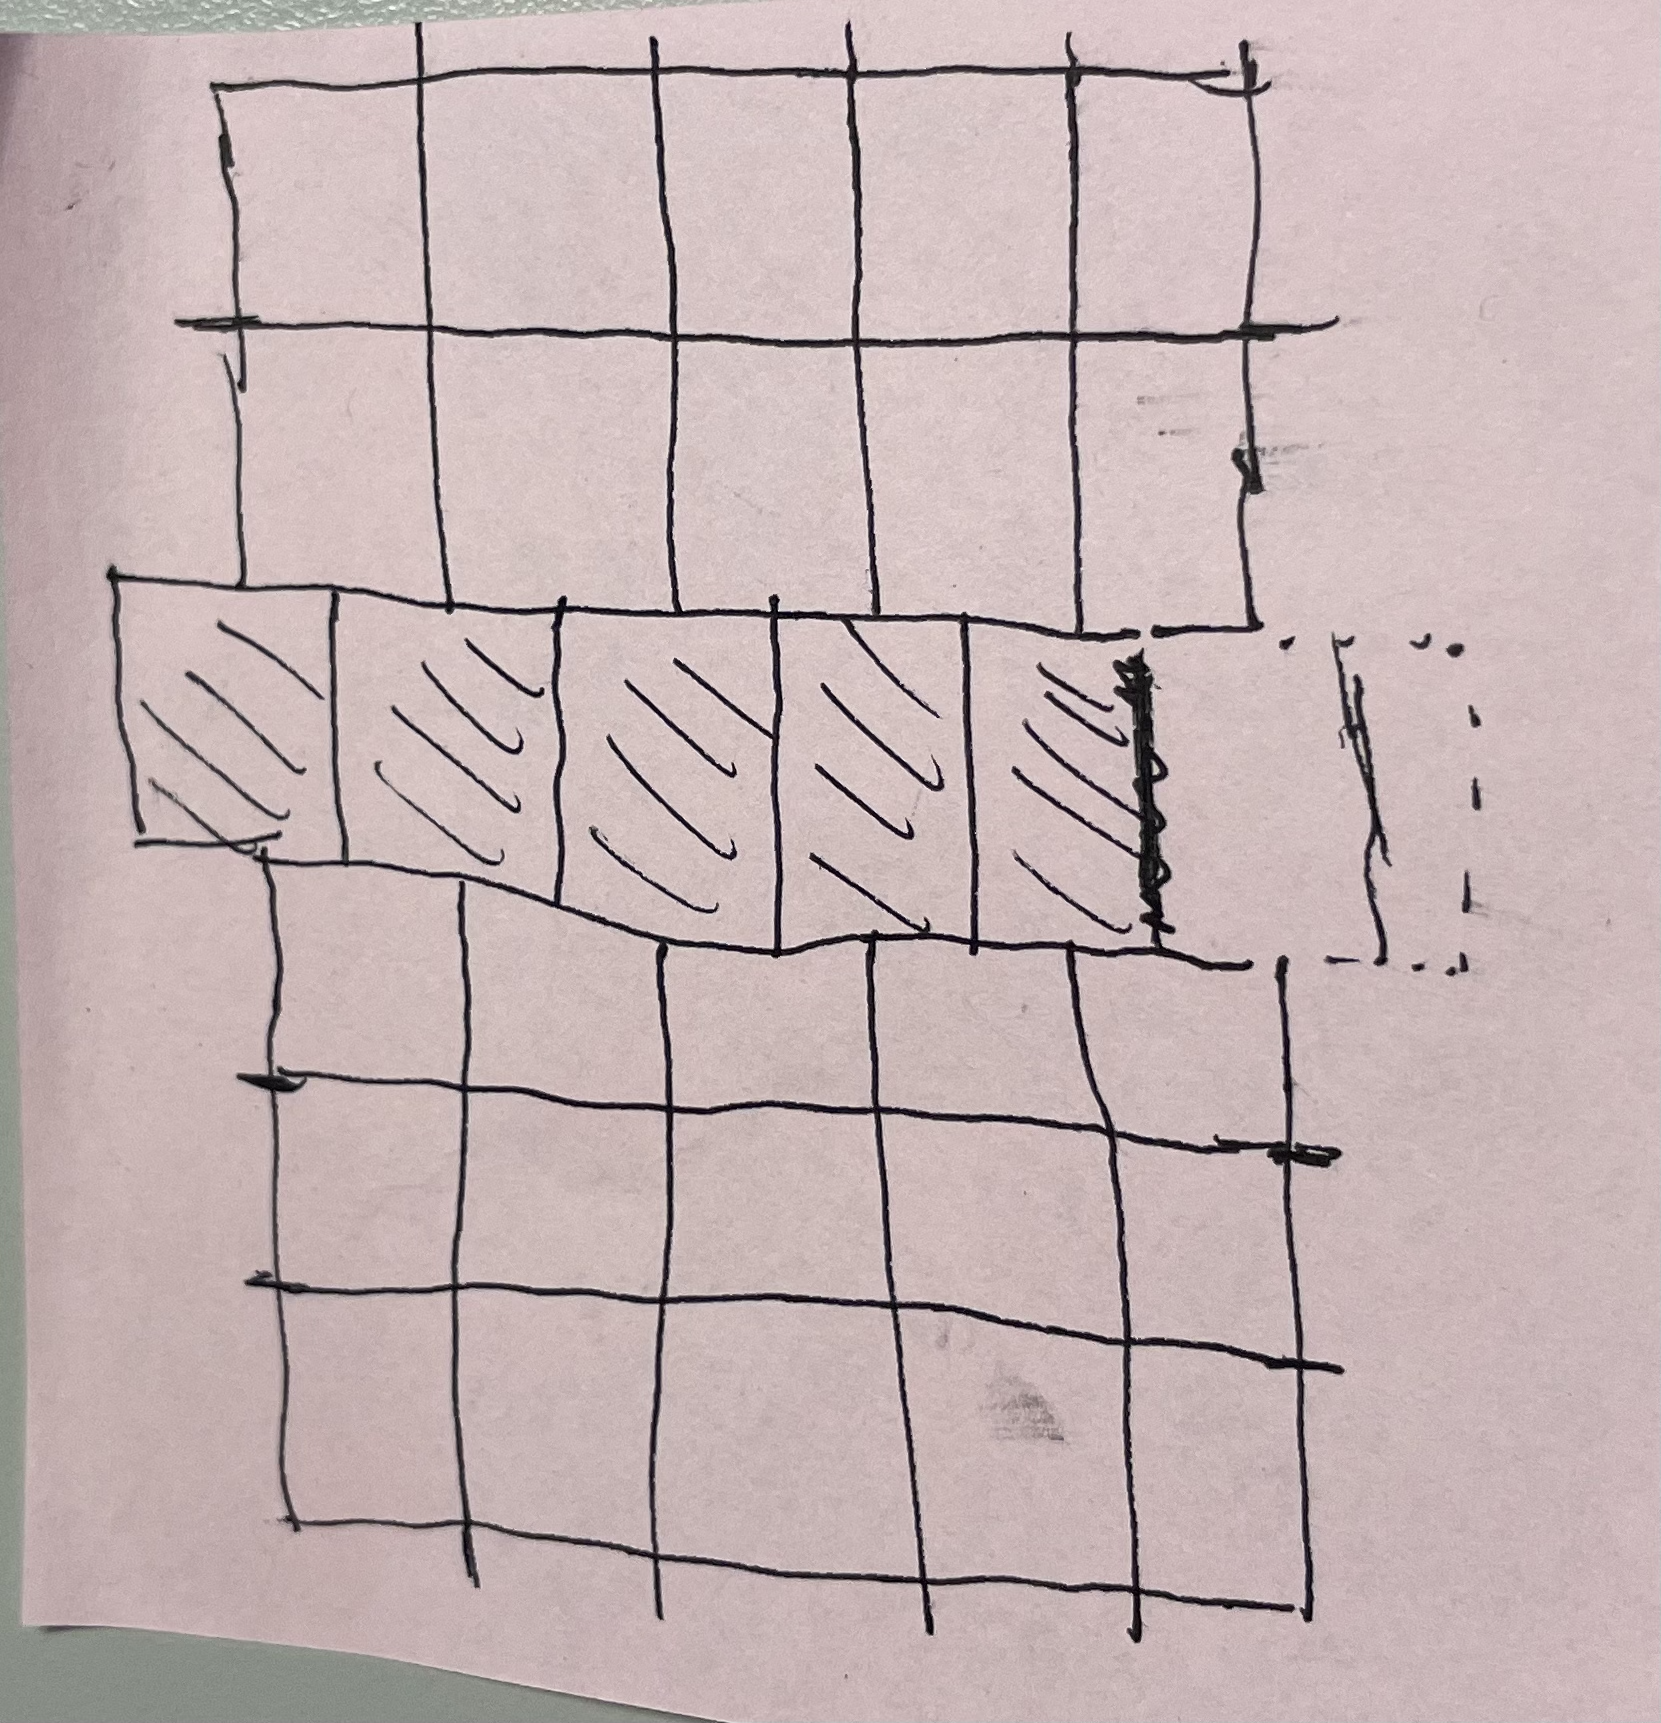
\includegraphics[width=0.9\linewidth]{single_shift_horizontal.png}
        \caption{Single shift horizontal}
        \label{fig:single_shift_horizontal}
    \end{subfigure}\quad
    \begin{subfigure}{.47\textwidth}
        \centering
        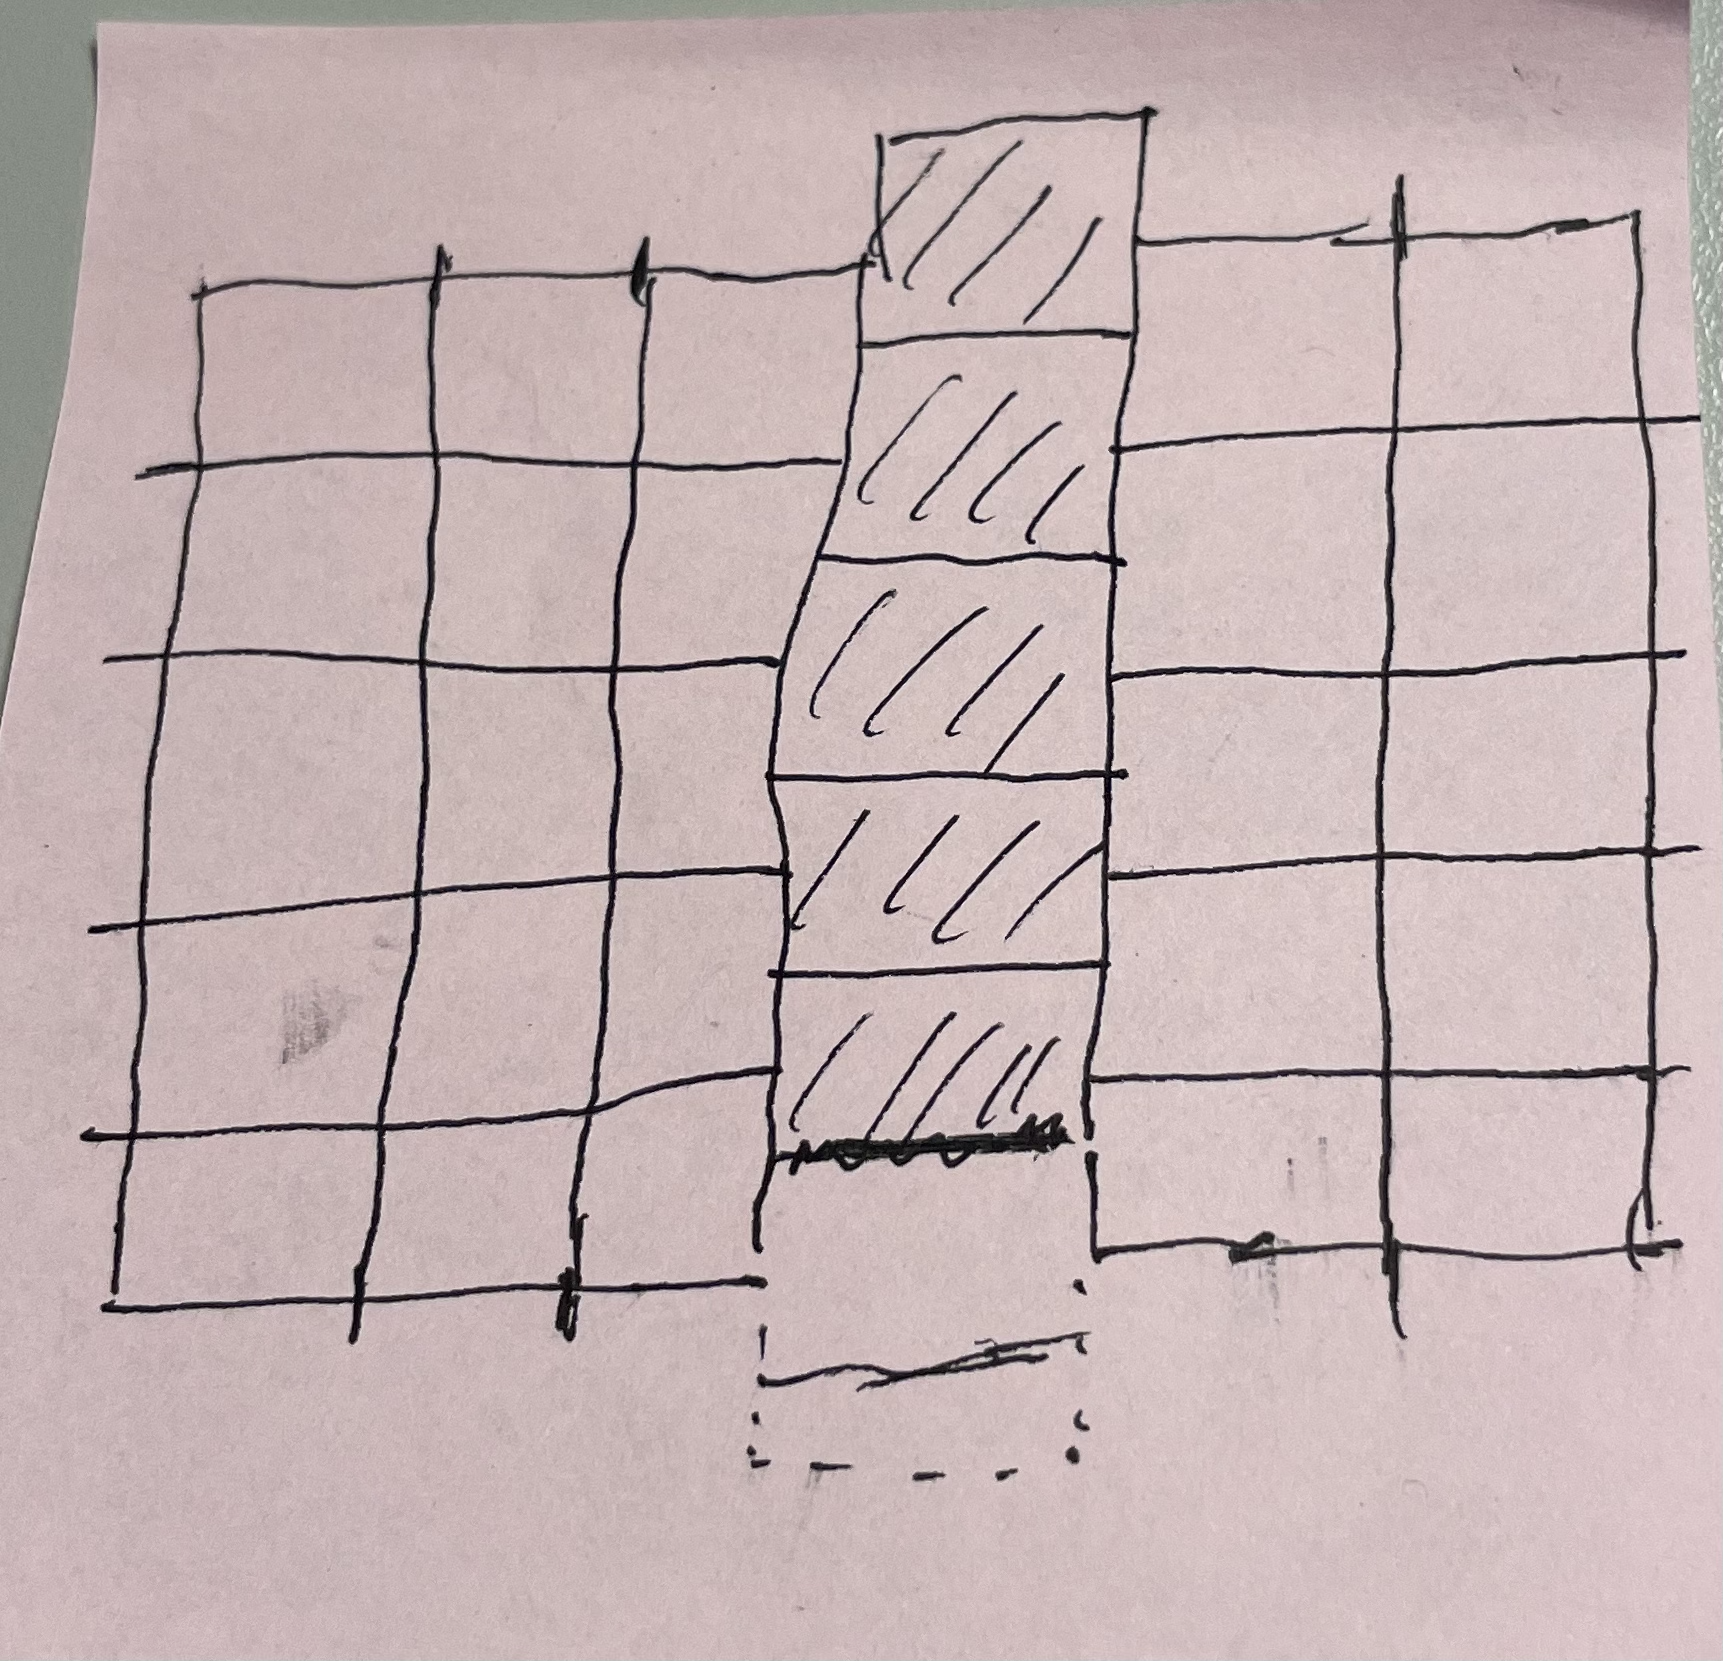
\includegraphics[width=0.9\linewidth]{single_shift_vertical.png}
        \caption{Single shift vertical}
        \label{fig:single_shift_vertical}
    \end{subfigure}\\
    \begin{subfigure}{.47\textwidth}
        \centering
        \includegraphics[width=0.9\linewidth]{same_shift_horizontal.png}
        \caption{same shift horizontal}
        \label{fig:same_shift_horizontal}
    \end{subfigure}\quad
    \begin{subfigure}{.47\textwidth}
        \centering
        \includegraphics[width=0.9\linewidth]{same_shift_vertical.png}
        \caption{same shift vertical}
        \label{fig:same_shift_vertical}
    \end{subfigure}\\
    \begin{subfigure}{.47\textwidth}
        \centering
        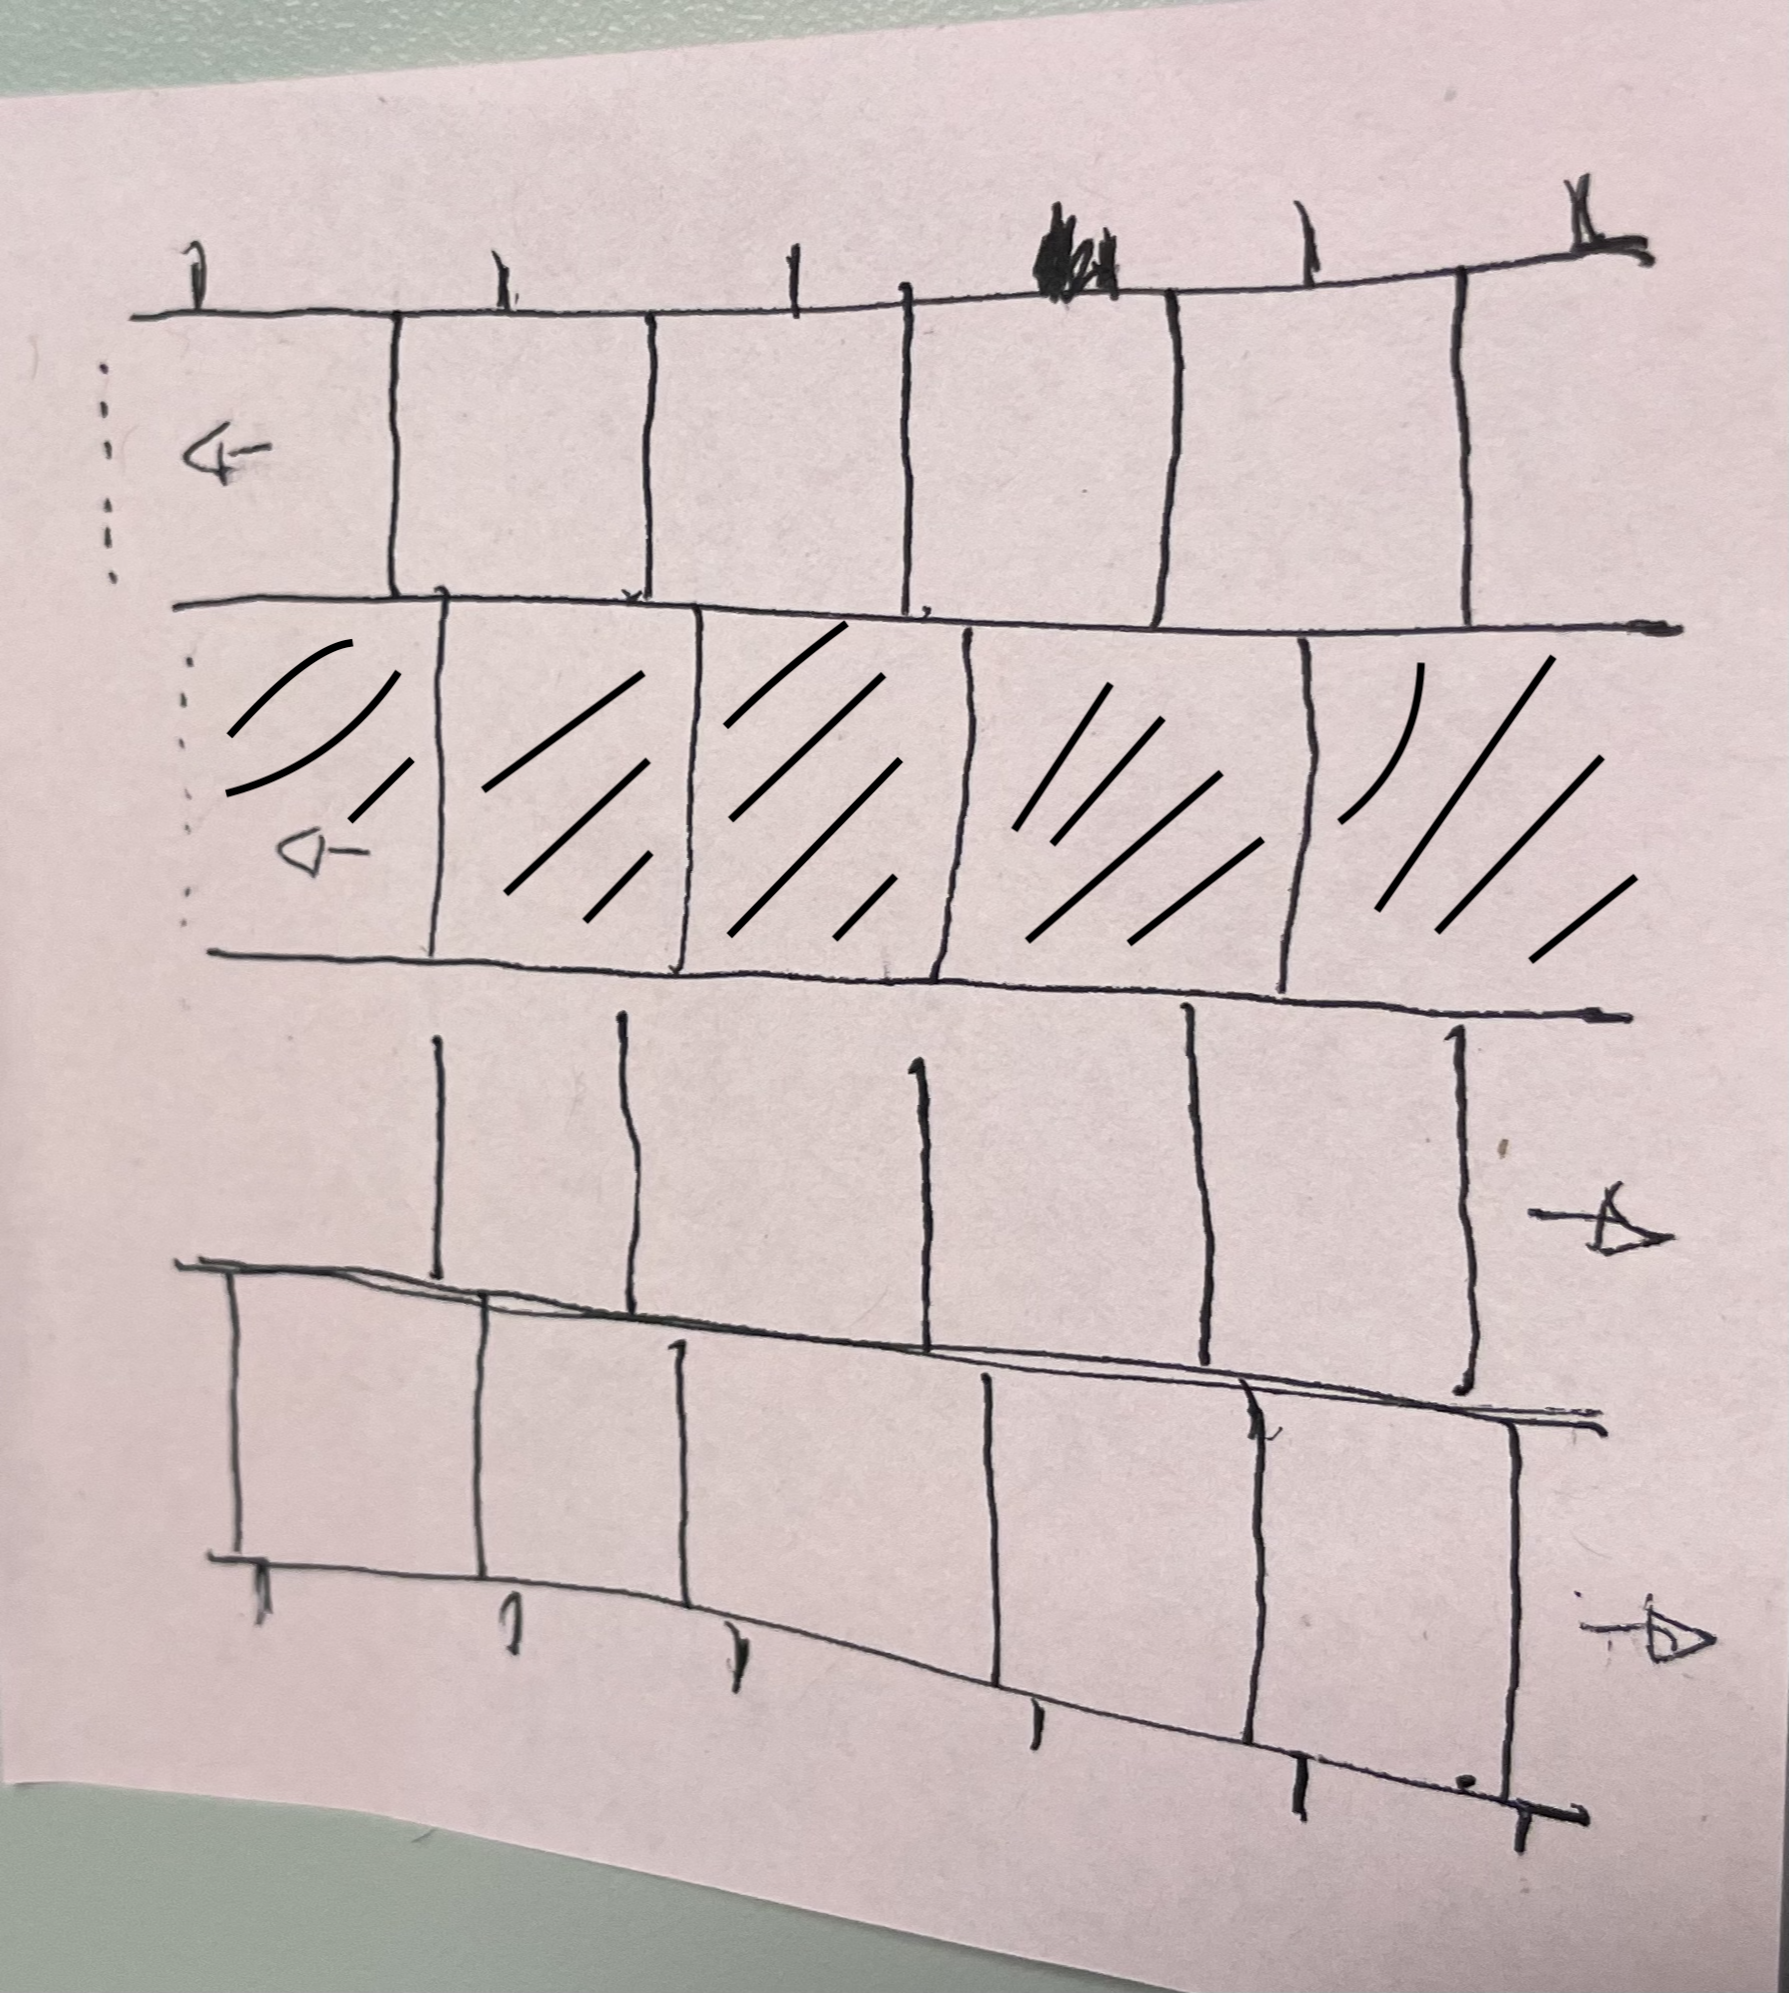
\includegraphics[width=0.9\linewidth]{multiple_shift_horizontal.png}
        \caption{Multiple individual shifts horizontal}
        \label{fig:multiple_shift_horizontal}
    \end{subfigure}\quad
    \begin{subfigure}{.47\textwidth}
        \centering
        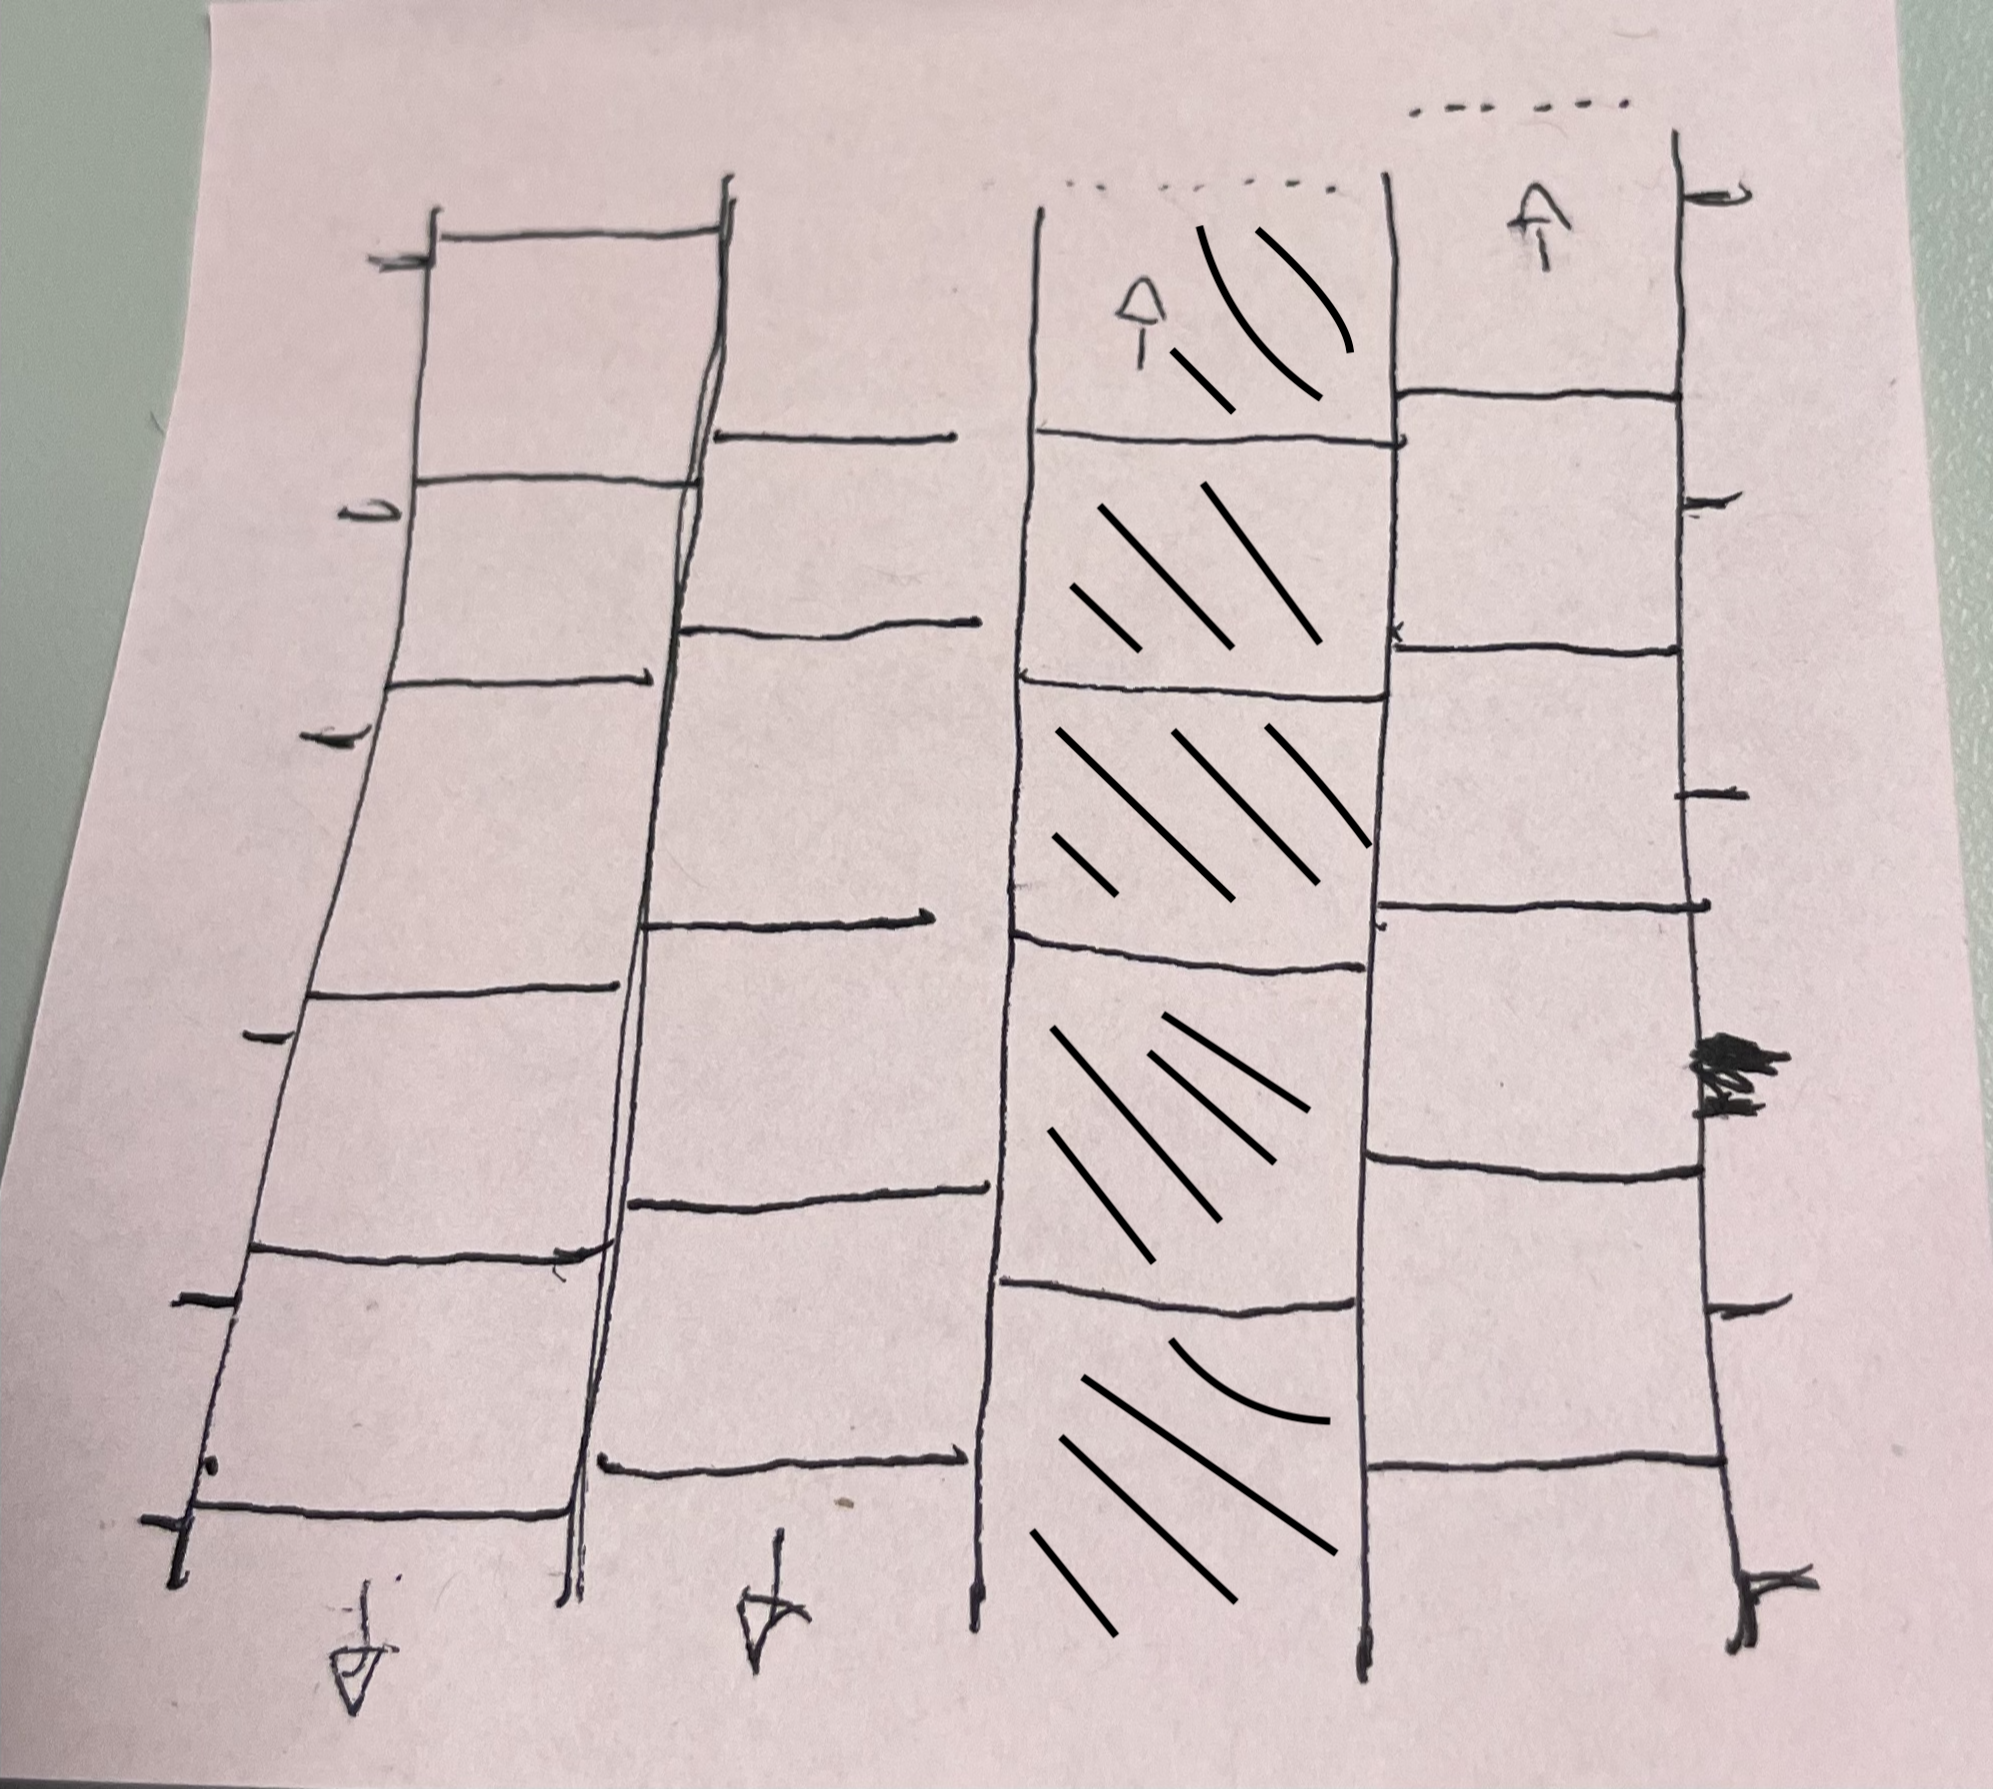
\includegraphics[width=0.9\linewidth]{multiple_shift_vertical.png}
        \caption{Multiple individual shifts vertical}
        \label{fig:multiple_shift_vertical}
    \end{subfigure}
    \caption{Different shifts}
    \label{fig:different_shifts}
\end{figure}

\begin{figure}[]%h!
    \centering
    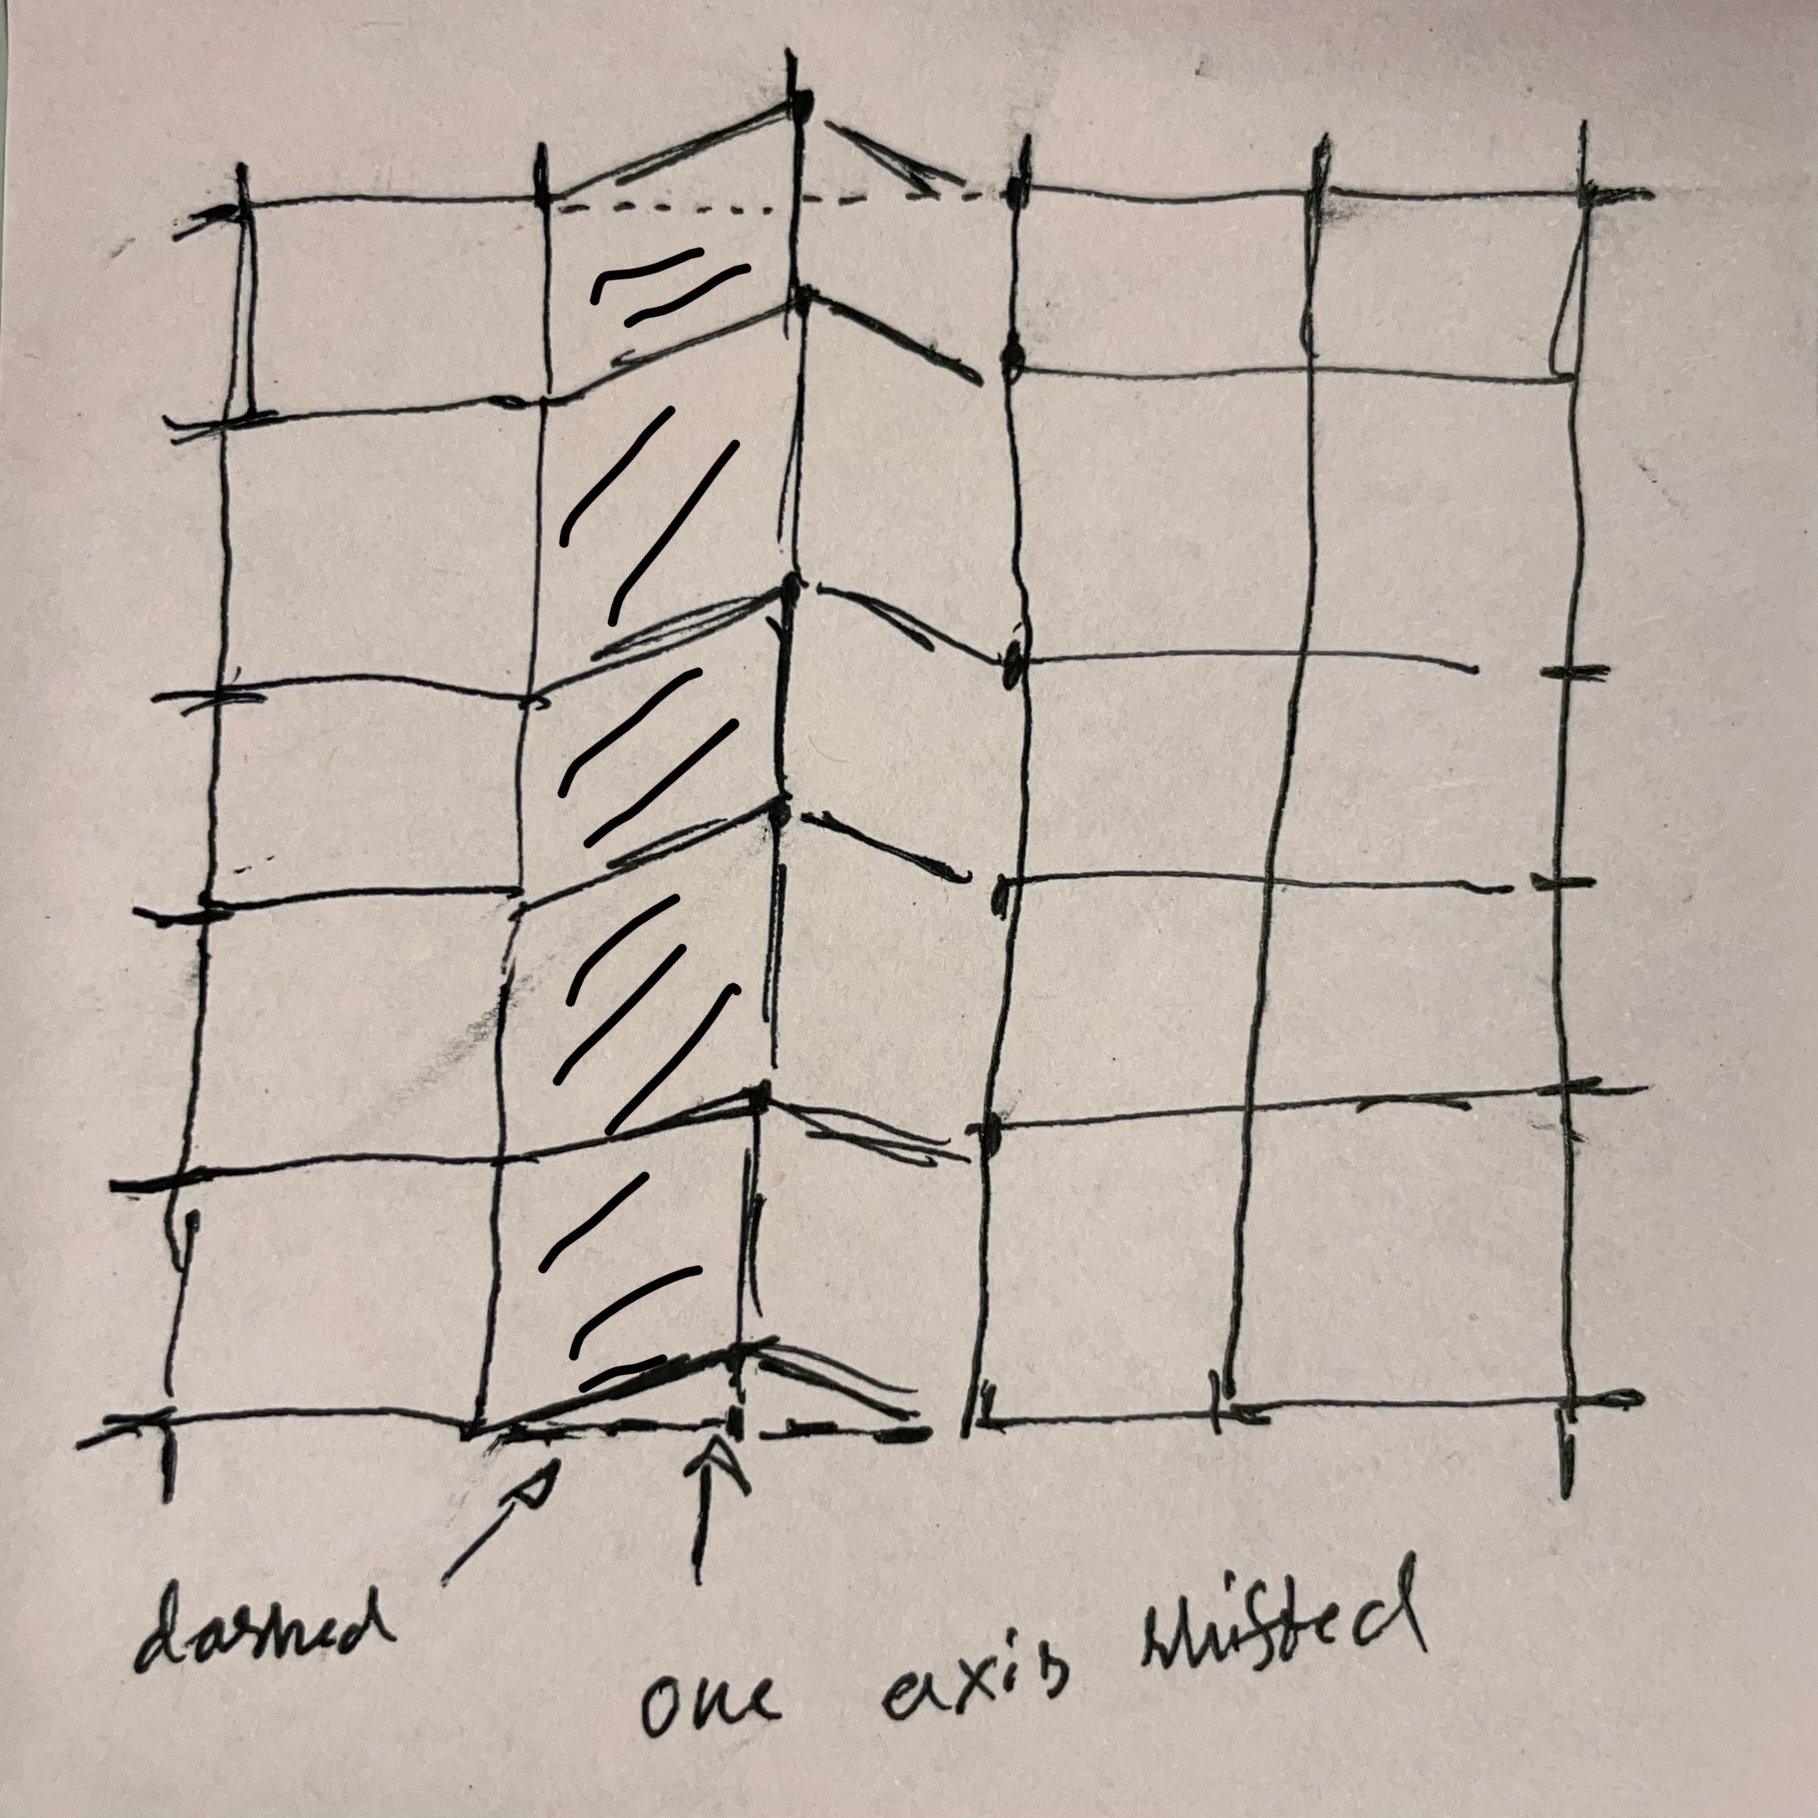
\includegraphics[width=0.45\linewidth]{legal.png}
    \caption{Dette er ikke helt riktig måte å tegne enkel skift på, hvorfor ikke?}
    \label{fig:not_allowed}
\end{figure}


\SigridComment{Eksplisitt vise at denne også er et skift, eller fokusere på theorem 3.2 i JorgensenPedersen som den vil følge fra (mtp, at jeg allerede har nesten gjort dette tidligere). Hvis det siste, kan den heller bruke for å ekseplifisere $\Lambda$ i to dimensjoner ved å linke den til illustrasjonene i figuren, samt lage noen flere for de andre}
\begin{align*}
    \Lambda(\lambda_1) = \begin{cases}        
        \mathbb{Z} & \text{for all } \lambda_1 \in \Lambda_1 \text{ except one}\\        
        \mathbb{Z}+\alpha & \text{for the one, where } \alpha \in \mathbb{R}   
    \end{cases}
\end{align*}

As with \cref{prop:class_all_shift}, we can classify all spectra in dimension two as follows. This significant result was proven by Pedersen and Jorgensen in the same paper \cite{jorgensenSpectralPairsCartesian2001}. 

\SigridComment{De nevner $\alpha$ bare som en index, og et "random" tall (ikke R), samt det virker mer som de indekserer med $m,n$ heller en $\alpha$, og det er heller ikke indeks på $\Lambda$ i seg selv for å få frem hva slags skift vi har}
\begin{theorem}\label{thrm:class_all_shift_2d}
    %$\braq{\beta_m \in [0,1) : m \in \Z}$ ANDRE skrivemåten for beta_m
    For a fixed $\alpha \in \R$ and an infinite sequence $\brac{\beta_m}_{m\in \Z}^\infty$, $\beta_m \in [0,1)$, the only subsets $\Lambda \subset \R^2$ such that $\Lambda$ is a spectrum for $I^2$ are either one of the two classes:
    \begin{equation}
        \Lambda = \braqMed{
            \begin{pmatrix}
            \alpha + m\\
            \beta_m + n
            \end{pmatrix} : m,n \in  \Z
            }
    \end{equation}
    or
    \begin{equation}
        \Lambda = \braqMed{
            \begin{pmatrix}
            \beta_n + m\\
            \alpha + n
            \end{pmatrix} : m,n \in  \Z
            }
    \end{equation}
    \SigridComment{ekskludert delen om at det også er et tiling set, det er vel hensiktsmessik og splitte disse opp, og komme tilbake til det i neste del, for å så komme med fulle og hele theorem 3.2.} 
\end{theorem}

remark om hvorfor sequencen er essensiell i dette tilfellet for å klassifisere alle skiftene %, samenlignet bare med bare noen random skift


remark om at vi ikke kan ha skift i to retninger, tegne dette

\begin{proof}
    
\end{proof}



\end{document}